\documentclass[a4paper, 11pt]{article}
\usepackage[top=3cm, bottom=3cm, left=2.5cm, right=2.5cm]{geometry}
\usepackage{amsmath}
\usepackage{amsfonts}
\usepackage{graphicx}
\usepackage{psfrag}
\usepackage[utf8]{inputenc}
\usepackage[T1]{fontenc}
\usepackage[colorlinks=true, allcolors=blue]{hyperref}
\usepackage[ruled,vlined]{algorithm2e}
\usepackage{tabto}
\usepackage{caption}

\title{Experimental Study Report : Knapsack Problem}
\author{Pierre BONNEFOY, Ophélie MARECHAL, Ian RIVIERE,\\
        Alexandre MARINE, Aloys LANA}



\begin{document}

\maketitle


\section{Abstract}

The knapsack problem is a very common NP problem. For this reason, we try today to solve it using different approaches. Basically, the problem is set like this :\par
\textit{Given a list of objects such that an object has a profit \textbf{p} and a weight \textbf{w}. You are given a knapsack with a maximum weight capacity \textbf{W}.} \\
The objective here is to maximize the profit of all objects that we can fit into the maximum capacity of the knapsack.\\
We solved this problem in 0/1 constraints, and for some algorithms in Multidimensional constraints.\\
To do this, we try all those different approaches :\\
\tabto{1.5cm} - Ant colony\\
\tabto{1.5cm} - Branch and bound\\
\tabto{1.5cm} - Brute force\\
\tabto{1.5cm} - Dynamic programming\\
\tabto{1.5cm} - Fully polynomial time approximation scheme\\
\tabto{1.5cm} - GRASP\\
\tabto{1.5cm} - Greedy (all)\\
\tabto{1.5cm} - Personal approach (meet-in-the-middle tweaked version)\par 
Then we will try to study the different results of each approach in order to find which approach was the best considering three factors:
\tabto{1.5cm} - Time complexity
\tabto{1.5cm} - Space complexity
\tabto{1.5cm} - Solution accuracy

\newpage

\tableofcontents



\section{Introduction}

In order to solve the knapsack problem, we first took the time to create a knapsack problem generator, capable of creating 0/1 knapsack problems, in order to grant us an infinite batch of files to work on. We also included some well-known databases to work on, namely :\\
\tabto{1.5cm} For 0/1 knapsack problems.\\
\tabto{2.5cm} - low-dimensional and large-scale from \href{http://artemisa.unicauca.edu.co/~johnyortega/instances_01_KP/}{Johny Ortega}
\tabto{1.5cm} For Multidimensional problems.\\
\tabto{2.5cm} - gk from \href{https://www.researchgate.net/publication/271198281_Benchmark_instances_for_the_Multidimensional_Knapsack_Problem}{F. Glover and G. Kochenberger}
\tabto{2.5cm} - chubeas from \href{https://www.researchgate.net/publication/271198281_Benchmark_instances_for_the_Multidimensional_Knapsack_Problem}{P. C. Chu and J. E. Beasley}

\newpage

\section{Working Organisation}
    \subsection{Tasks Repartition}
    \begin{center}
        \captionof{table}{Table representing the repartition of the tasks for each member of the group.}
        \begin{tabular}{|p{4cm}|p{2cm}|}
            \hline
            \textbf{Task} & \textbf{Name} \\
            \hline
            Generator & Ian RIVIERE\\
            \hline
            Terminal main & Alexandre MARINE\\
            \hline
            Interface & Pierre BONNEFOY \\
            \hline
            Generation of analysis graphics. & Ophélie MARECHAL \\
            \hline
            Ant Colony fo 0/1 problems. & Pierre BONNEFOY \\
            \hline
            Branch and Bound for 0/1 problems. & Ophélie MARECHAL \\
            \hline
            Brute Force for 0/1 problems.  & Aloys LANA \\
            \hline
            Dynamic Programming for 0/1 problems. & Ian RIVIERE \\
            \hline 
            FPTAS for 0/1 problems. & Ian RIVIERE \\
            \hline
            GRASP for 0/1 problems.  & Alexandre MARINE \\
            \hline
            Greedy for 0/1 problems.  & Alexandre MARINE \\
            \hline
            GRASP for Multidimensional problems.  & Alexandre MARINE \\
            \hline
            Greedy for Multidimensional problems.  & Alexandre MARINE \\
            \hline
            Brute Force for Multidimensional problems.  & Aloys LANA \\
            \hline
        \end{tabular}
    \end{center}

    \newpage

    \subsection{Planification}
    \begin{center}
        \captionof{table}{Table representing the planification of the project and the status of the tasks.}
        \begin{tabular}{|p{2cm}|p{8cm}|p{2cm}|}
            \hline
            \textbf{Deadline} & \textbf{Task} & \textbf{State} \\
            \hline
            \hline
            21/10/2022 & Writing the Group Description, Planification and Task Repartition. & Done \\
            \hline 
            28/10/2022 & Definition of the format used for the generator files. Developement of the Knaspack Problem Generator. & Done \\
            \hline
            10/11/2022 & Each member will have implemented one method on 0/1 Knapsack Problems. & Done \\
            \hline
            17/11/2022 & All algorithm are implemented on 0/1 Knapsack Problems & Done \\
            \hline 
            30/11/2022 & The study of algorithm is started and the Brute Force, Greedy, GRASP are implemented for Multidimensional Knapsack Problems. & Done \\
            \hline
            04/12/2022 & Graphic Interface finished. & Done \\
            \hline
            07/12/2022 & Study Report is finished and upload of the final version. & Done \\
            \hline
        \end{tabular}
    \end{center}

\section{Implementation Choices}
    \subsection{Ant Colony}

    We choose to set two variables \verb+MINPHERO+ and \verb+MAXPHERO+ to 0.01 and 6 respectively as they are the registered values of this \href{https://hal.archives-ouvertes.fr/hal-01541529/document}{study archive}.\\
    After some test from Pierre's on his own, he spotted that those parameters weren't really impactful in opposition to these next variables : \verb+ALPHA+, \verb+RHO+ and \verb+BETA+.\\
    \verb+ALPHA+ corresponds to how important pheromones will be for ants.\\
    \verb+RHO+ corresponds to the evaporation ratio of pheromones.\\ 
    \verb+BETA+ corresponds to how important the ratio of objects profit and weight is for ants.\\
    Those variables are set such that $\verb+ALPHA+ = 2$, $\verb+RHO+ = 0.98$ and $\verb+BETA+ = 5$ and were determined by the scientists of the study. After a lot of test from Pierre, he confirms that those values are the most optimized parameters for working with ants.\\
    Only those five variables comes from the study alongside their method for computing the probability as Pierre already wrote the algorithm and was already getting some interesting results on all test files.\\
    Then he chose to not implement the more accurate version of the study as the results granted with the ratio calculus were good enough.
  

    \subsection{Branch and Bound}
    For the branch and bound agorithm, in order to try to optimize the space complexity and the execution time, we decided that rather than creating an entire tree, the algorithm only consider the information concerning the current node (a set of objects, its value and weight) and the best solution found (a final set of objects, the final value and the final weight), which is equivalent to a leaf of the tree.\\
    This way, the algorithm will browse the list of objects and for each of them, try to take it or not, which is similar to the brute force approach. But the particularity of the branch and bound algorithm is that if the best of the remaining objects compose a solution which is worse than current best, the exploration of these items can be ignored, which allows a large calculation reduction.\\
    The two set of objects are represented by tables which are filled with a 0 if the object at this index isn't taken, and 1 if it's taken.
    
    

    
    \subsection{Brute Force}
    The brute force algorithm is going through all the possibile solutions so in order to try to optimize the execution speed, we made two choices : 
    \tabto{1.5cm} - Generation of all the possibilities by using a list of all the \verb+N+ binary combinations, where \verb+N+ corresponds to the number of object of the problem. Each bit, corresponds to the status of the object : a value of 1 means that the object is in the Knapsack and a value of 0 means that it isn't in. For example, with \verb+N+ = 2 we obtain the following result : [[0,0],[0,1],[1,0],[1,1]]. This allow us to not going through all the Object List at each iteration. \\
    \tabto{1.5cm} - Reduction of the calculations, if the weight of the current possibilty is outrunning the Knapsack Capacity, we stop going through this possibility and we go through the next one.\\
    \tabto{1.5cm} - By the same idea, we reduce the number of calculation for Multidimensional Knapsack Problems, if the weight of the current possibilty of this dimension is outrunning the Knapsack Capacity of this dimension, we stop going trough this possibility and we go through the next one.
    
    \subsection{Dynamic Programming}

    The dynamic programming approach was implemented using our courses. This means that we divide the problem into smaller problems and we keep track of all values found until the end in a matrix created like that : $matrix[n][m]$ with $n$ the number of items and $m$ all possible weigth.\par
    While checking for all objects if the object weight exceed the maximum capacity, we ignore it. But if it could fit, we check if it's value is of greater interest than the last one included. If yes, we then include it, otherwise we don't.\par

    After this we built a Truth list to check which item was included.



    \subsection{Fully polynomial time approximation scheme}

    We were asked to implement a fully polynomial time approach, the easiest way for us was from upgrading the dynamic approach.\par
    The dynamic approach has a big flaw, it runs way better on smaller value, and tends to slow down when the profit becomes bigger.\par
    That's where the fptas approach shines the best, by reducing the profits to value between 0 and 9. We can speed up the dynamic algorithm by a lot. In order to do so, we check for the higher power of 10 objects in the list. After this we can build an auxiliary list of objects but with value restricted to the sets \verb+{0,1,2,3,4,5,6,7,8,9}+.\par 
    However this should mean that we can't get all objects back from the dynamic processing (as all objects were reduced and we couldn't guess which object was the first with value 1 for example). In order to prevent that, we loose some space complexity optimization by creating a list of indexes of all objects included, so that we can find them way easier after the dynamic procees.


    \subsection{GRASP}

    For our random approach we choose to work with GRASP methodology. It consists of running a Greedy approach but in order to try to optimize the final value we take a random object between $x$ objects, x being a value that we choose. As it is random, the process will run $t$ times the random version of greedy.\par
    This allow us to change how accurate the algorithm can be, for instance we choose to set it to 3. This makes the algorithm run a little bit random as we choose randomly between 3 items, but it stills allow us to reach the optimal choice as it is between the 3 best choices at this time of the computation.\par
    If we tweak this parameter to take more objects for the choice, we will make the algorithm runs more randomly but by extension, we could devalue the final result as we could make a choice that isn't really efficient at this time of the computation.\par
    In order to try to find the optimal value, we need to choose how many iterations per run are processed. Most commonly this number is $t = 10$, but since we saw that most files were running fast enough, we set it to 30, this allowed us to prevent some cases where the algorithm didn't found the optimal value because of a lack of luck basically.\par
    For the multidimensional constraints, as we are built around the greedy approach there isn't anything different from this methodology.

    \subsection{Greedy}

    For the greedy approach, even if we had to build three different versions based on the selector, we ended up building the same sorting method.
    So we have those three versions :
    \tabto{1.5cm} - Greedy by value : sorting using the value of objects.\\
    \tabto{1.5cm} - Greedy by weight : sorting using the wieght of objects.\\
    \tabto{1.5cm} - Greedy : sorting using the ratio of object value divide by object weigth.\par

    For sorting all objects, we choose to use the \verb+TIMSORT+ sorting methods.
    It consists of mixing the insertion sort and the merge sort to increase it's speed. We first need to divide the list of objects into smaller groups of size such that $size\_sub\_list \in G$ such that $G = \{all\ number\ based\ on\ a\ power\ of\ two\}$. We set the minimal value to 32.\par
    
    For the Multidimensional constraints, there isn't a lot of change with 0/1 constraints. We only change the weight calculus to take all dimensions into account.


    \subsection{Personal approach}

    We needed to think of a personal approach that isn't one already asked. That's where the brute force comes handy, as we could already see from the tests used as implementation validation for all algorothms (to be certain they all worked as intended). We could already spot the weakness of brute force.\par
    That's when Alexandre got an idea, he thoughs of an adaptation of the divide and conquer algorithm called \verb+meet-in-the-middle+.\par
    This methodology consists of splitting the input list of objects in two, and find all subsets for both half-list. Because the brute force algorithm was already built, we simply call it on both of those sub list, and then we choose the best object and the second sub list, in order to add them into the first until we can't anymore.

\section{Tests}
    \subsection{Test procedure}

    Every tests were made following this protocol :
    It was done on a laptop with those specifications :
    \tabto{1.5cm} - Processor AMD Ryzen 5 4600H
    \tabto{2.5cm} -- 6 cores and 2 sockets (12 virtual cores) running at 4Ghz
    \tabto{1.5cm} - architecture x86\_64
    \tabto{1.5cm} - 8 GiB of RAM running at 3200MHz

    Only the process \verb+launcher.py+ was launched during the test periods (at the exception of all daemon process and the terminal).

    For the ant colony and GRASP, all values are a median of multiple tests (10 runs per Algo), to ensure that we approximate the best way the value as it includes some randomness.

    We decided to split the algorithms that have similar functioning into 4 Categories in order to make the tests :
    \tabto{1.5cm} - Brute Force, Branch and Bound and Personnal approach
    \tabto{1.5cm} - Dynamic Programming and FPTAS
    \tabto{1.5cm} - Ant Colony and GRASP
    \tabto{1.5cm} - Greedies algorithms
    
    Once we had determined the best of each category, we have been able to test around the 4 remaining algorithms to determine the best one.

    \subsection{Test Results on 0/1 Problems}
        \subsubsection{Time Complexity}
        \begin{center}
            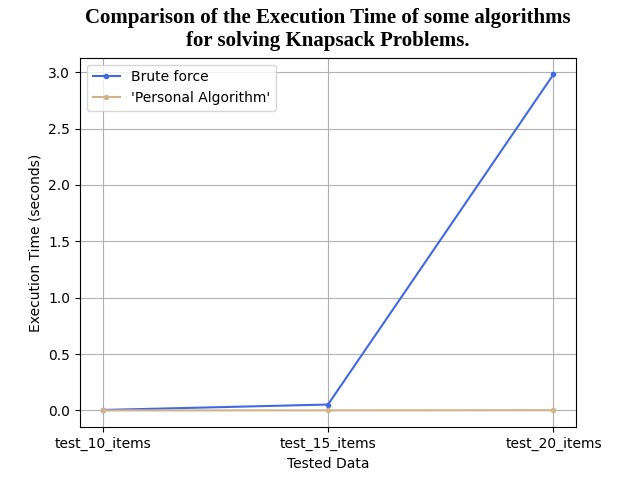
\includegraphics[scale = 0.5]{graph_bf_perso.png}
            \captionof{figure}{Comparison between Brute Force and Personal Algorithm}
            
            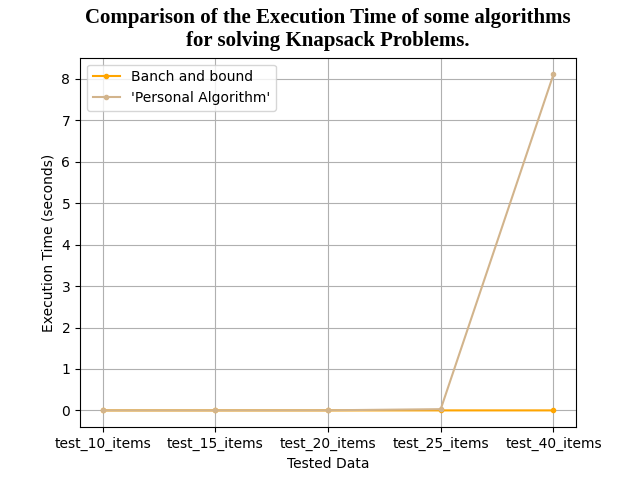
\includegraphics[scale = 0.5]{graph_perso_bab.png}
            \captionof{figure}{Comparison between Personal Algorithm and Branch and Bound}
            
            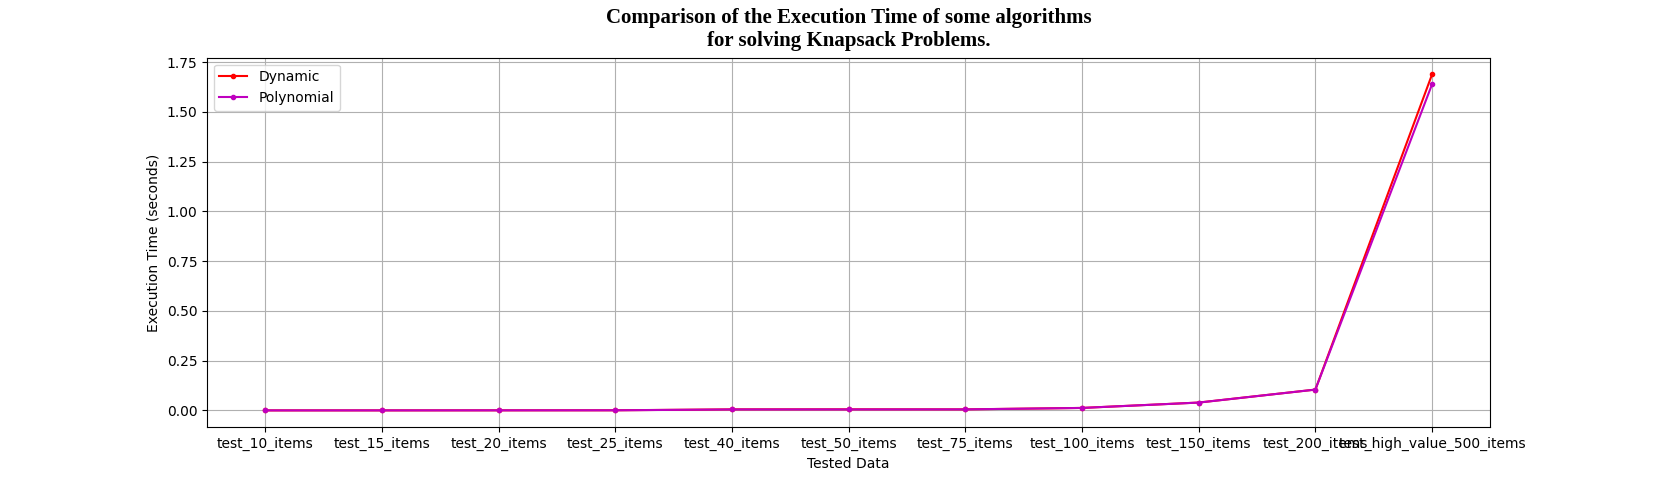
\includegraphics[scale = 0.4]{graph_dyna_poly.png}
            \captionof{figure}{Comparison between Dynamic Programming and FPTAS}
            
            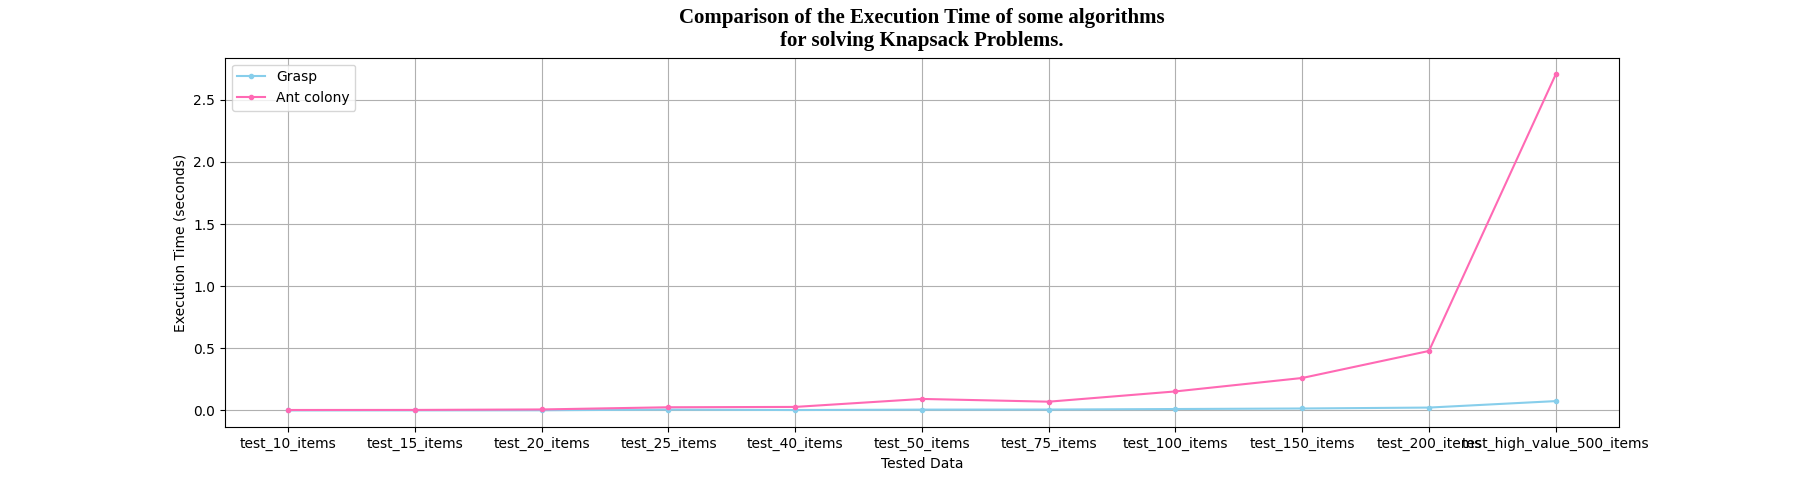
\includegraphics[scale = 0.4]{graph_grasp_ant.png}
            \captionof{figure}{Comparison between Ant Colony and GRASP}
            
            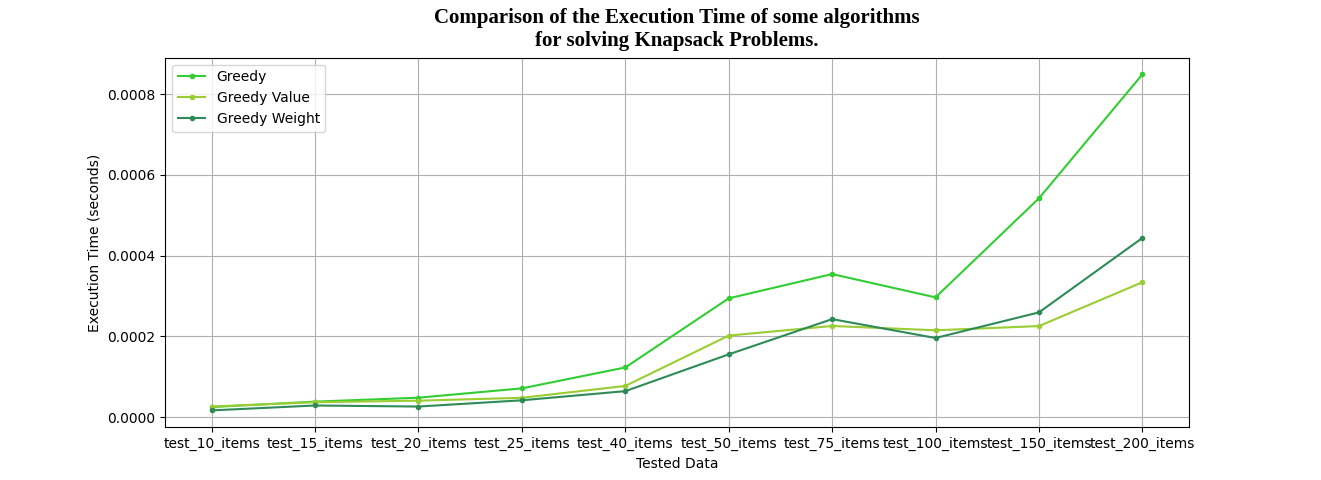
\includegraphics[scale = 0.5]{graph_greedys.png}
            \captionof{figure}{Comparison between Greedies algorithms}
            
            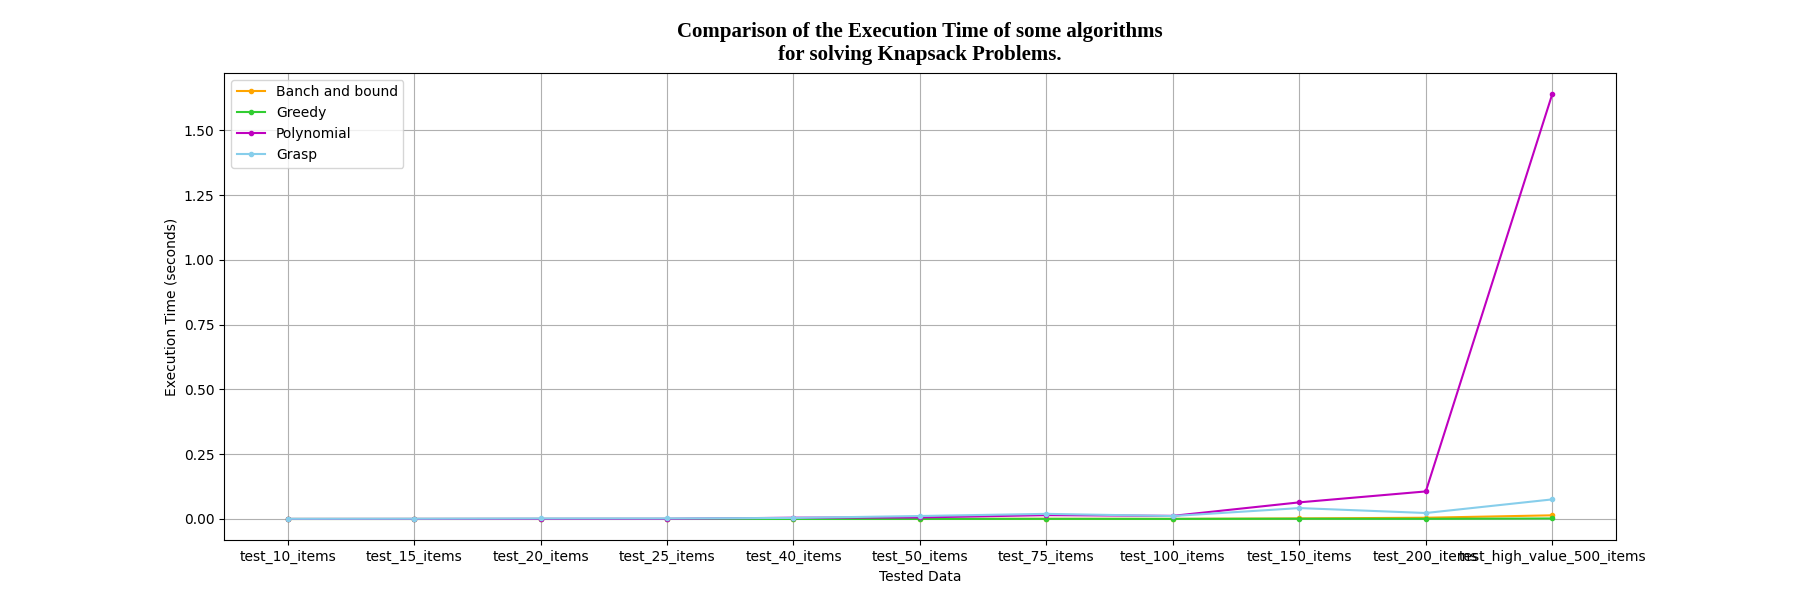
\includegraphics[scale = 0.4]{graph_bests.png}
            \captionof{figure}{Comparison between the Best One of Each Category}

            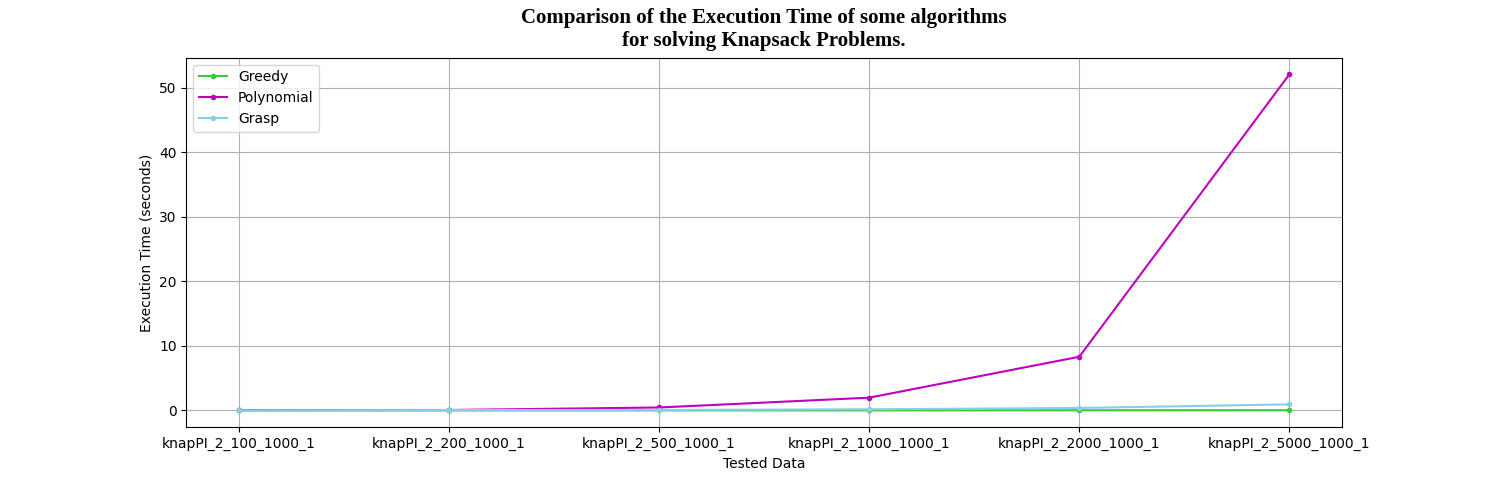
\includegraphics[scale = 0.5]{graph_high_numbers.png}
            \captionof{figure}{Comparison between GRASP, all greedy and polynomial}

            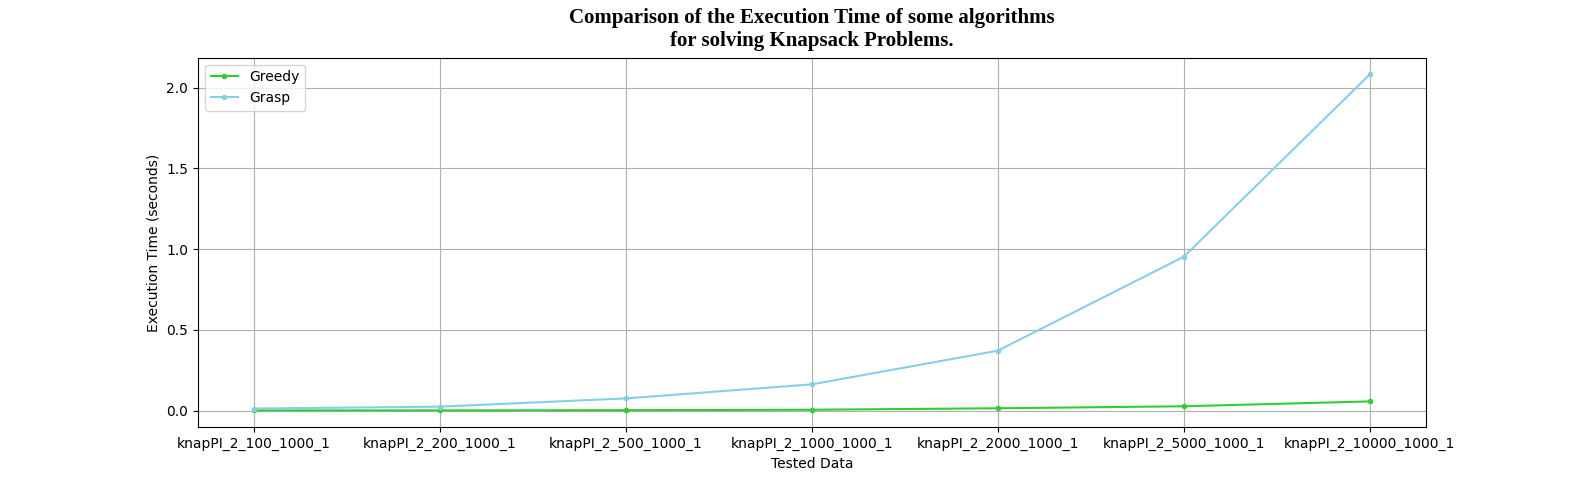
\includegraphics[scale = 0.5]{graph_best_high_numbers.png}
            \captionof{figure}{Comparison of the two best at very high numbers.}
        \end{c}
        \subsubsection{Solution Accuracy}


            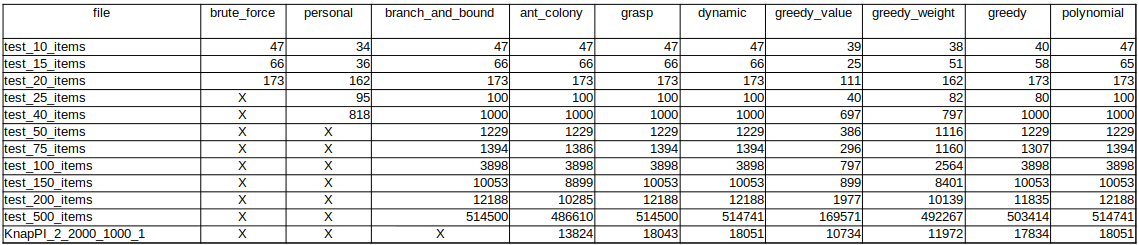
\includegraphics[scale = 0.45]{values_0-1.png}
            \captionof{figure}{}

    \subsection{Test Results on Multidimensional Problems}

    \subsubsection{Time Complexity}

    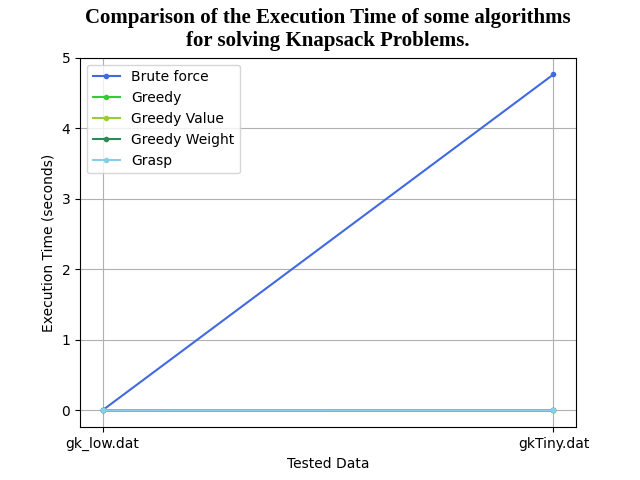
\includegraphics[scale = 0.5]{graph_multi_1.png}
    \captionof{figure}{Comparison between GRAPS, Brute Force and all Greedy}

    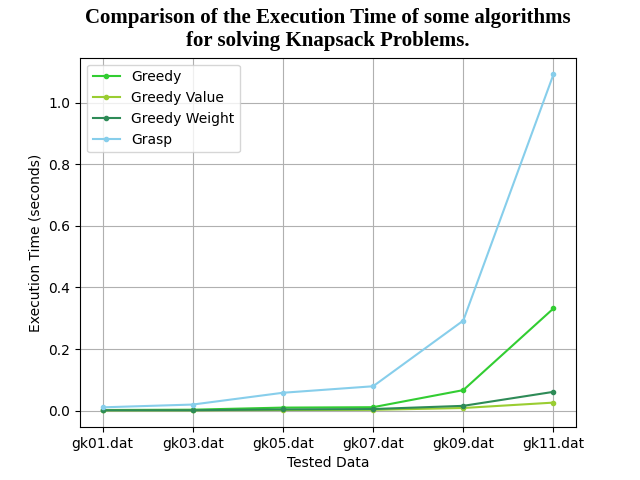
\includegraphics[scale = 0.5]{graph_multi_gk_greed.png}
        \captionof{figure}{Comparison between GRASP and all Greedy}


    \subsubsection{Accuracy}

    \subsection{Results Interpretation}
       

\section{Workload}
\begin{center}
    \captionof{table}{Table representing the Workload in percentage for each group member.}
    \begin{tabular}{|p{2cm}|p{2cm}|}
        \hline
        \textbf{Name} & \textbf{Percentage} \\
        \hline
        \hline
        Alexandre MARINE &  35\% \\
        \hline 
        Pierre BONNEFOY &  20\% \\
        \hline
        Ian RIVIERE & 15\% \\
        \hline
        Ophélie MARECHAL &  15\% \\
        \hline 
        Aloys LANA &  15\% \\
        \hline
    \end{tabular}
\end{center}

\section{Conclusion}

\newpage

\appendix
\section{Annexes}

\listofalgocfs
\newpage

\subsection{Algorithms}
\begin{algorithm}[hbt!]
    \caption{Branch\_and\_Bound}\label{alg:two}
    \KwData{$listItems$ : Item list, $nbItems$ : Number of items, $w$ : Capacity of the knapsack}
    \KwResult{$finalItems$ : Solution item list, $finalValue$ : Solution value}
    
    \BlankLine
    \textbf{Global} $NB\_ITEMS$, $W$, $finalWeight$, $finalValue$, $finalSolution$, $tempSolution$\\
    
    \BlankLine
    \tcc{Initialisation}
    $NB\_ITEMS \leftarrow nbItems$ ; 
    $W \leftarrow w$\\
    \textbf{sort $listItems$ by value/weight}\\
    $finalWeight \leftarrow 0$ ; 
    $finalValue \leftarrow 0$ ; 
    $finalSolution \leftarrow []$\\
    $currentWeight \leftarrow 0$ ; 
    $currentValue \leftarrow 0$ ; 
    $tempSolution \leftarrow []$\\
    \While{$len(tempSolution) < NB\_ITEMS$}{
    $tempSolution.append(0)$
    }
    
    \BlankLine
    \tcc{Call of the recursive function}
    $Branch\_and\_Bound\_Recursive(listItems,currentValue, currentWeight, 0)$
    
    \BlankLine
    \tcc{Returned data}
    fill $finalItems$ list with the items selected in $finalSolution$ (where $finalSolution[i] == 1$)\\
    \Return $finalItems, finalValue$
    
    
\end{algorithm}

\begin{algorithm}[hbt!]
    \caption{Branch\_and\_Bound\_Recursive}\label{alg:two}
    \KwData{$listItems$ : Item list, $currentWeight$ : Weight of the current solution, $currentValue$ : Value of the current solution, $i$ : index of the current item}
    \KwResult{fill $finalWeight$, $finalValue$ and $finalSolution$}
    
    \BlankLine
    \textbf{Global} $NB\_ITEMS$, $W$, $finalWeight$, $finalValue$, $finalSolution$, $tempSolution$\\
    
    \BlankLine
    \tcc{If the current item $i$ can be taken}
    \If{$currentWeight + listItems[i][1] \leq W$}{
        $tempSolution[i] \leftarrow 1$\\
        \If{$i < NB\_ITEMS-1$}{
            $Branch\_and\_Bound\_Recursive(listItems, currentValue + listItems[i][0], currentWeight + listItems[i][1], i+1)$
        }
        \If{($i = NB\_ITEMS-1)$ \textbf{and} $(currentValue + listItems[i][0] > finalValue)$}{
            $finalValue \leftarrow currentValue + listItems[i][0]$\\
            $finalWeight \leftarrow currentWeight + listItems[i][1]$\\
            $finalSolution \leftarrow tempSolution$\\
        }
    }
    

    \BlankLine
    \tcc{If the following items can lead to a better solution}
    \If{$Bound(listItems, currentValue, currentWeight, i) \geq finalValue$}{
        $tempSolution[i] \leftarrow 0$\\
        \If{$i < NB\_ITEMS-1$}{
            $Branch\_and\_Bound\_Recursive(listItems,currentValue, currentWeight, i+1)$
        }
        \If{($i = NB\_ITEMS-1)$ \textbf{and} $(currentValue > finalValue)$}{
            $finalValue \leftarrow currentValue$ ; 
            $finalWeight \leftarrow currentWeight$\\
            $finalSolution \leftarrow tempSolution$\\
        }
    }

\end{algorithm}

\newpage

\begin{algorithm}[hbt!]
    \caption{Bound}\label{alg:two}
    \KwData{$listItems$ : Item list, $currentWeight$ : Weight of the current solution, $currentValue$ : Value of the current solution, $i$ : index of the current item}
    \KwResult{$v$ : Maximum value reachable using the items following the current item $i$}
    
    \BlankLine
    \textbf{Global} $NB\_ITEMS$, $W$\\
    
    \BlankLine
    $v \leftarrow currentValue$\\
    $w \leftarrow currentWeight$\\
    
    \BlankLine
    \For{$j \leftarrow i+1\ \KwTo\ NB\_ITEMS$}{
        \If{$w + listItems[j][1] \leq W$}{
            $w \leftarrow w + listItems[j][1]$\\
            $v \leftarrow v + listItems[j][0]$\\
        }
    }

\Return{$v$}	
\end{algorithm}

\newpage


    \begin{algorithm}[hbt!]
        \SetKw{In}{in}
        \SetKw{Break}{break}
        \SetKw{Continue}{continue}
        \caption{GenerateAllPossibilities}
        \label{alg_brute_force_GenerateAllPossibilities}
        \KwData{n : Number of bits}
        \KwResult{List of every sequence of n bits possible.}
        \BlankLine
        $l \longleftarrow [[0], [1]]$\;
        $start \longleftarrow 0$\;
        \BlankLine
        \For{$i \longleftarrow 1$ \KwTo $n$}{
            $tmp \longleftarrow len(l)$\;
            \For{$element$ \In $l[start:]$}{
                $l \longleftarrow l.append([0] + element)$\;
                $l \longleftarrow l.append([1] + element)$\;
            }
            $start \longleftarrow tmp$\;
        }
        \Return{$l[start:]$}
        \BlankLine
    \end{algorithm}

        \begin{algorithm}[hbt!]
            \SetKw{InEnumerate}{in enumerate}
            \SetKw{Break}{break}
            \caption{Brute Force for 0/1 Knapsack Problems}
            \label{alg_brute_force_0/1}
            \KwData{maxWeigth : Capacity of the Knapsack, objectList : List of object of the problem.}
            \KwResult{Final Knapsack, Final Value}
            \BlankLine
            $allPossibilities \longleftarrow GenerateAllPossibilities(len(objectList))$\;
            $currentBest \longleftarrow (0, -1)$\;
            \BlankLine
            \For{$currentPossibility, element$ \InEnumerate $allPossibilities$ }{
                $currentWeigth \longleftarrow 0$\;
                $currentValue \longleftarrow 0$\;
                \For{$index, bit$ \InEnumerate $element$}{
                    \If{$bit == 1$}{
                        $currentWeigth \longleftarrow currentWeigth + objectList[index][1]$\;
                        \eIf{$currentWeigth <= maxWeigth$}{
                            $currentValue \longleftarrow currentValue + objectList[index][0]$\;
                        }
                        {
                            \Break
                        }
                    }
                \If{$currentValue > currentBest[1]$}{
                    $currentBest \longleftarrow (currentPossibility, currentValue)$\;
                }
                }
            }
            \tcc{Reconstitution Of Knapsack for Displaying Purposes.}
            $finalKnapsack \longleftarrow []$\;            
            \For{$i, obj$ \InEnumerate $allPossibilities[currentBest[0]]$}{
                \If{$obj == 1$}{
                    $finalKnapsack \longleftarrow finalKnapsack.append([objectList[i]])$\;
                }
            }
            \Return{$finalKnapsack, currentBest[1]$}
            \BlankLine
        \end{algorithm}

    \newpage

        \begin{algorithm}[hbt!]
            \SetKw{InEnumerate}{in enumerate}
            \SetKw{Break}{break}
            \SetKw{Continue}{continue}
            \caption{Brute Force for Multidimensional Knapsack Problems}
            \label{alg_brute_force_Multidimensional}
            \KwData{ksc : List of the capacity of each dimension of the Knapsack, objectList : List of object of the problem.}
            \KwResult{Final Knapsack, Final Value}
            \BlankLine
            $allPossibilities \longleftarrow GenerateAllPossibilities(len(objectList))$\;
            $currentBest \longleftarrow (0, -1)$\;
            $nbDimension \longleftarrow len(ksc)$\;
            \BlankLine
            \For{$currentPossibility, element$ \InEnumerate $allPossibilities$ }{
                $currentWeigth \longleftarrow initializeWith0(nbDimension)$\;
                $currentValue \longleftarrow 0$\;
                \For{$index, bit$ \InEnumerate $element$}{
                    \If{$bit == 1$}{
                        \For{$dimension \longleftarrow 0$ \KwTo $nbDimension$}{
                            $currentWeigth[dimension] \longleftarrow currentWeigth[dimension] + objectList[index][1][dimension]$\;

                            \If{$not(currentWeigth <= maxWeigth)$}{
                                \Break
                            }
                        }
                        \Else{
                            $currentValue \longleftarrow currentValue + objectList[index][0]$\;
                            \Continue
                        }
                        \Break
                    }
                \If{$currentValue > currentBest[1]$}{
                    $currentBest \longleftarrow (currentPossibility, currentValue)$\;
                }
                }
            }
            \BlankLine
            \tcc{Reconstitution Of Knapsack for Displaying Purposes.}
            $finalKnapsack \longleftarrow []$\;            
            \For{$i, obj$ \InEnumerate $allPossibilities[currentBest[0]]$}{
                \If{$obj == 1$}{
                    $finalKnapsack \longleftarrow finalKnapsack.append([objectList[i]])$\;
                }
            }
            \Return{$finalKnapsack, currentBest[1]$}
            \BlankLine
        \end{algorithm}

\newpage

\begin{algorithm}
    \caption{Greedy}
    \DontPrintSemicolon
    \SetKwFunction{FMain}{Main}
    \SetKwProg{Fn}{Function}{:}{}
    \KwData{$list\_objects$, $wmax$,  a list of tuple object  with their profit and weight and the maximum capacity of the knapsack.}\;
    \Fn{\FMain{$list\_objects$, $wmax$}}{
        $start\_timer$\;
        $list\_temp \gets list\_objects[:]$\;
        $cw \gets wmax$\;
        $final\_list\_objects \gets []$\;
        $final\_value \gets 0$\;

        $timsort(list\_temp)$\;

        \For{$i$ \KwTo{len($list\_temp$)}}{
            \eIf{$cw - list\_temp[i][1] > 0$}{
                $cw -= list\_temp[i][0]$\;
                $fw += list\_temp[i][0]$\;
                $final\_knapsack.append(list\_temp[i])$\;
            }{
                $break$\;
            }
        }
        $end\_timer$\;
    }
        
    \KwResult{$time\_taken$, $final\_knapsack$, $final\_value$}\;

    \SetKwFunction{FTimsort}{Timsort}
    \Fn{\FTimsort{$list\_objects$}}{
        $n \gets len(list\_objects)$\;
        $minrun \gets find\_minrun(n)$\;

        \For{$start \gets minrun$ \KwTo{n}}{
            $end \gets min(start + (minrun-1), n-1)$\;
            $insertion\_sort(list\_objects, start, end)$\;
        }
        $size \gets minrun$\;
        \While{$size < n$}
        {
            \For{$left \gets 2*size$ \KwTo{$n$}}
            {
                $mid \gets min(n-1, (left + size-1))$\;
                $right \gets min( (left + 2 * size - 1), n-1)$\;

                \If{$mid < right$}{
                    $merge(list\_objects, left, mid, right)$\;
                }
            }
            $size \gets 2 * size$\;
        }
        \KwResult{$sorted\_list$, the input list sorted.}
    }\;

    \SetKwFunction{FFindMinrun}{Find\_minrun}
    \Fn{\FFindMinrun{$n$}}{
        $r \gets 0$\;
        \tcc{ \textit{MINIMUM is set globally to 32}}
        \While{$n >= MINIMUM$}{
            $r \gets$ $n | 1$\;
            \tcc{\textit{Binary OR comparison between the bits value of n and 1}}\;
            $n \gets >> 1$\;
            \tcc{\textit{Binary shifting of the bits value of 1. Corresponds to dividing n by 2**1}}\;
        }
        \KwResult{$minimal\_run\_size$, the runnable size that will be used to split the lists. Will always be a power of 2.}
    }

\end{algorithm}


\begin{algorithm}
    \SetKwProg{Fn}{Function}{:}{}
    \caption{Greedy (follow up)}
    \DontPrintSemicolon

    \SetKwFunction{FInsertsort}{Insertion\_sort}
    \Fn{\FInsertsort{$list\_objects$, $left$, $right$}}{
        \For{$i$ \textbf{from} $left + 1$ \KwTo{$right + 1$}}{
            $j = i$\;
            \While{$j > left$ \textbf{and} $list\_objects[j][0]/list\_objects[j][1] > list\_objects[j - 1][0]/list\_objects[j-1][1]$}{
                $list\_objects[j]$, $list\_objects[j-1] \gets list\_objects[j-1]$, $list\_objects[j]$\;
                $j--$\;
            }
        }
    }
    \KwResult{$sorted\_list$, using insertion methods on the left and right parts of input.}\;


    \SetKwFunction{FMerge}{Merge}
    \Fn{\FMerge{$list\_objects$, $left$, $mid$, $right$}}{
            $len1 \gets mid - left + 1$\;
            $len2 \gets right - mid$\;

            $left\_part$, $right\_part \gets []$\;

            \For{$i \gets 1$ \KwTo{$len1$}}{
                $left.append(list\_objects[left + i])$\;
            }

            \For{$i \gets 1$ \KwTo{$len2$}}{
                $right.append(list\_objects[mid + 1 + i])$\;
            }

            $i$, $j \gets 0$\;
            $k \gets left$\;

            \While{$i < len1$ \textbf{and} $j < len2$}{
                \eIf{$left\_part[i][0]/left\_part[i][1]$ $<$ $right\_part[j][0]/right\_part[j][1]$}{
                    $list\_objects[k] \gets  right\_part[j]$\;
                    $j++$\;
                }
                {
                    $list\_objects[k] \gets left\_part[i]$\;
                    $i++$\;
                }
                $k++$\;
            }
            \While{$i < len1$}{
                $list\_objects[k] \gets left\_part[i]$\;
                $k++$\;
                $i++$\;
            }
            \While{$j < len2$}{
                $list\_objects[k] \gets right\_part[j]$\;
                $k++$\;
                $j++$\;
            }
        }
        \KwResult{$merged\_list$, a sorted version of list\_objects based on a merge version of it's left and right parts.} 
\end{algorithm}

\newpage

\begin{algorithm}
\SetKwProg{Fn}{Function}{:}{}
\caption{GRASP}
\DontPrintSemicolon
\KwData{$list\_objects$, $nbI$, $wmax$,  a list of tuple object  with their profit and weight, the number of Iterations and the maximum capacity of the knapsack.}\;

\SetKwFunction{FMain}{Main}
\Fn{\FMain{$list\_objects$,$nbI$,$wmax$}}{
    $start\_timer$\;
    $final\_list$, $final\_value \gets grasp(list\_objects$, $nbI$, $wmax)$\;
    $end\_timer$\;
}
\KwResult{$time\_taken$, $final\_knapsack$, $final\_value$}\;

\SetKwFunction{FGrasp}{GRASP}
\Fn{\FGrasp{$list\_objects$,$nbI$,$wmax$}}{
    $best \gets 0$\;
    $list\_temp \gets []$\;
    $solution \gets []$\;
    $v \gets 0$\;
    \For{$i$ \KwTo{$nbI$}}{
        $list\_temp$, $v \gets greedy\_randomised\_construction(list\_objects$, $wmax)$\;

        \If{$v > best$}{
            $best \gets v$\;
            $solution \gets liste\_temp[:]$\;
        }
    }
}
\KwResult{$solution$, $best$}\;

\SetKwFunction{FGrandom}{Greedy\_randomised\_construction}
\Fn{\FGrandom{$list\_objects$, $wmax$}}{
    $list\_temp \gets list\_objects[:]$\;
    $cw \gets wmax$\;
    $final\_list \gets []$\;
    $final\_value \gets 0$\;
    $timsort(list\_temp)$\;
    \While{$len(list\_temp > 0$}{
        $current\_candidates \gets []$\;
        \For{$i$ \KwTo{3}}{
            \If{$i < len(list\_temp)$}{
                $current\_candidates.append(list\_temp[i])$\;
            }
        }
        $chosen\_object \gets random.choice(current\_candidates)$\;
        \If{$chosen\_object[1] <= cw$}{
            $final\_list.append(chosen\_object)$\;
            $cw -= chosen\_object[1]$\;
            $final\_value += chosen\_object[0]$\;
        }
        $list\_temp.pop(list\_temp.index(chosen\_object[0]))$\;
    }
}
\KwResult{$final\_list$, $final\_value$}\;

\end{algorithm}

\newpage


\begin{algorithm}[hbt!]
    \caption{Ant Colony}\label{alg:two}
    \KwData{$list\_objects, nb\_ant, nb\_objects, wmax$}
    \KwResult{$best\_solution['objects'], best\_solution['value']$}
    $init\_phero(phero)$\;
    $best\_solution \leftarrow \{'num\_object' = [],'objects' = [], 'value' = -1, 'weight' = -1\}$\;
    \For{$ant=1\ \KwTo\ nb\_ant $}{
        $current\_solution \leftarrow \{'num\_object' = [],'objects' = [], 'value' = -1, 'weight' = -1\}$\;
        $init\_candidates(candidates, list\_objects)$\;
        $check \leftarrow 0$\;
        $current \leftarrow 0$\;
        $set\_probabilities(probabilities,phero,list\_objects,candidates,current)$\;
        $x \leftarrow\ random\ between\ 0\ and\ 1$\;
        \ForEach{$i\ in\ probabilities$}{
            \If{$x \in i$ \textbf{and} $current\_solution['weight']+list\_objects[i['num\_object']]['weight']<=wmax$}{
                $remove\ i['num\_object']\ of\ candidates$\;
                $remove\ i['num\_object']\ of\ probabilities$\;
                $add\ list\_objects[i['num\_object']]\ to\ current\_solution$\;
                $current \leftarrow i['num\_object']$\;
                $check \leftarrow check\ +\ 1$\;
            }
        }
        \While{$check \neq nb\_objects$}{
            $et\_probabilities(probabilities,phero,list\_objects,candidates,current)$\;
            $x \leftarrow random\ between\ 0\ and\ 1$\;
            \ForEach{$i\ in\ probabilities$}{
                \eIf{$x \in i$ \textbf{and} $current\_solution['weight']+list\_objects[i['num\_object']]['weight']<=wmax$}{
                    $remove\ i['num\_object']\ of\ candidates$\;
                    $remove\ i['num\_object']\ of\ probabilities$\;
                    $add\ list\_objects[i['num\_object']]\ to\ current\_solution$\;
                    $current \leftarrow i['num\_object']$\;
                    $check \leftarrow check\ +\ 1$\;
                }{
                    \If{$current\_solution['weight']+list\_objects[i[num\_object]]['weight']<=wmax$}{
                        $remove\ i['num\_object']\ of\ candidates$\;
                        $remove\ i['num\_object']\ of\ probabilities$\;
                        $check \leftarrow check\ +\ 1$\;
                    }
                }
            }
        }
        \If{$current\_solution['value']>best\_solution['value']$}{
            $best\_solution \leftarrow current\_solution$ \;
        }
        $update\_phero(phero)$\;
        $set\_phero(phero,best\_solution,current\_solution)$\;
    }
\end{algorithm}

\newpage

\begin{algorithm}
    \caption{Dynamic programming}
    \DontPrintSemicolon
    \SetKwFunction{FMain}{Dynamic programming}
    \SetKwProg{Fn}{Function}{:}{}
    \KwData{$list\_objects$, $wmax$, a list of tuple object with their profit and weight, the maximum capacity of the knapsack}

    \Fn{\FMain{$list\_objects$,$wmax$}}{
        $start\_timer$\;
        $list\_temp \gets list\_objects$\;
        $final\_list \gets []$\;
        $final\_value \gets 0$\;
    
        \tcc{Creating the matrix of 0 to n objects as rows and 0 to Knapsack max weight}\;

        $matrix = [0] *\ (w+1)\ *\ (len(list\_temp) + 1)$

        \tcc{Filling the table}\;
        \For{$i$ \KwTo $len(list\_temp) + 1$}{
            \For{$j$ \KwTo $wmax + 1$}{
                \uIf{$i == 0$ or $j == 0$}{
                    $matrix[i][j] \gets 0$\;
                }
                \uElseIf{$list\_temp[i-1][1] <= j$}{
                    $matrix[i][j] \gets max(list\_temp[i-1][0] + matrix[i-1][j - list\_temp[i-1][1]], matrix[i-1][j])$\;
                }
                \Else{
                    $matrix[i][j] \gets matrix[i-1][j]$\;
                }
            }
        }
        $final\_value = matrix[len(list\_temp)][wmax]$\;
        $checking\_value \gets final\_value$\;
        $checking\_weight \gets wmax$\;

        \tcc{Getting all selected items}\;
        \For{$i \gets -1$ \textbf{from} $len(list\_temp)$ \KwTo $0$}{
            \If{$checking\_value <= 0$}{
                $break$\;
            }
            \eIf{$checking\_value == matrix[i-1][checking\_weight]$}{
                $continue$\;
            }
            {
                $final\_list.append(list\_temp[i-1])$\;
                $checking\_value -= list\_temp[i-1][0]$\;
                $checking\_weight -= list\_temp[i-1][1]$\;
            }
        }


        $end\_timer$\;


}
\KwResult{$final\_list$, $final\_value$}

\end{algorithm}

\newpage

\begin{algorithm}

    \caption{Fully polynomial time approximation scheme}
    \DontPrintSemicolon
    \SetKwFunction{FMain}{Fptas}
    \SetKwProg{Fn}{Function}{:}{}

    \KwData{$epsilon$, $wmax$, $list\_objects$}

    \Fn{\FMain{$epsilon$, $wmax$, $list\_objects$}}{
        $start\_timer$\;
        $final\_value \gets 0$\;
        $final\_list \gets []$\;

        $P \gets list\_objects[0][0]$\;

        \For{$i$ \textbf{from} $1$ \KwTo{$len(list\_objects)$}}{
            \If{$list\_objects[i][0] > P$}{
                $P \gets list\_objects[i][0]$\;
            }
        }

        $K \gets (epsilon * P) / len(list\_objects)$\;

        $list\_temp \gets [(int(a[0]/K), a[1])\ for\ a \in list\_objects]$\;

        \tcc{It's a slightly modified version of Dynamic programming returning the list of index instead of the final\_list}
        $list\_index \gets dynamic(list\_temp, wmax)$\;

        \For{$i \in liste\_index$}{
            $final\_sac.append(list\_objects[i])$\;
            $final\_value += list\_objects[i][0]$\;
        }

        $end\_timer$\;
    }
    \KwResult{$final\_list$, $final\_value$}

    
\end{algorithm}

\newpage

\subsection{Checklist}
\begin{enumerate}
    \item Did you proofead your report?
    \item Did you present the global objective of your work?
    \item Did you present the principles of all the methods/algorithms used in your project?
    \item Did you cite correctly the references to the methods/algorithms that are not from your own?
    \item Did you include all the details of your experimental setup to reproduce the experimental results, and explain the choice of the parameters taken?
    \item Did you provide curves, numerical results and error bars when results are run multiple times?
    \item Did you comment and interpret the different results presented?
    \item Did you include all the data, code, installation and running instructions needed to reproduce the results?
    \item Did you engineer the code of all the programs in a unified way to facilitate the addition of new methods/techniques and debugging?
    \item Did you make sure that the results different experiments and programs are comparable?
    \item Did you sufficiently comment your code?
    \item Did you add a thorough documentation on the code provided?
    \item Did you provide the additional planning and the final planning in the report and discuss organization aspects in your work?
    \item Did you provide the workload percentage between the members of the group in the report?
    \item Did you send the work in time?
\end{enumerate}

\end{document}




    